\chapter{Úvod do problematiky}
V tejto kapitole si vysvetlíme základne pojmy potrebné pre túto bakalársku prácu.
\section{Biologické pozadie}
\subsection{DNA,Gén,Genóm}
\paragraph{DNA}
Deoxyribonukleová kyselina je nositeľom genetickej informácie bunky.\\
Má štruktúru dvojzávitnice, skladajúcej sa z dvoch komplementárnych vlákien.
Vlákno je tvorené nukleotidmy, ktoré obsahujú jednu zo štyroch báz Adenín,Guanín,Tymín a Cytozín.
DNA zvykneme zapisovať ako postupnosť týchto báz, kde každú bázu kódujeme jej počiatočným písmenom - A,G,T,C.

\paragraph{Gén}
Gén je súvislý úsek DNA ktorý kóduje tvorbu proteínu. Gén je základnou jednotkou dedičnosti.

\paragraph{Genóm}
Genóm je súbor DNA molekúl organizmu, ktoré sa väčšinou nachádzajú v chromozómoch.
Napríklad v ľudskom tele sa jedná o 46 molekúl DNA, jedna v každom chromozóme[6].
\subsection{Evolučná história}\label{evhist}
Evolučná história je postupnosť udalostí, ktoré sa odohrali na nejakej DNA sekvencii.
Pre potreby tejto práce sú podstatné udalosti odohrávajúce sa na dlhých úsekoch DNA - génoch.
\newline
Možné udalosti sú:
\newline
\begin{itemize}
\item \emph{Duplikácia} - skopírovanie génu na iné miesto v DNA.
\item \emph{Inzercia} - vloženie nového génu.
\item \emph{Delécia} - odstránenie génu.
\item \emph{Inverzia} - zmena poradia a orientácie génu alebo génov.
\item \emph{Translokácia} - zmena poradia génu alebo génov 
\item \emph{Speciácia} - špeciálna udalosť, ktorá označuje vznik nového druhu. Vzniká nová vetva v evolučnej histórii.
\end{itemize}
\subsubsection{Krok evolučnej histórie}
Krok evolučnej histórie, ďalej len \emph{krok e.h} je pre nás známa sekvencia génov. 
Medzi jednotlivími krokmi došlo k jednej alebo viacerím udalostiam. 

\subsection{Fylogenetický strom}
Fylogenetický strom je grafické znázornenie, ktoré zobrazuje evolučné vzťahy medzi sadou objektov. Pokiaľ si za objekty zvolíme druhy, jedná sa o takzvaný \emph{Druhový strom}.
Jednotlivé druhy sú pospájané hranami, ktoré reprezentujú evolučný vzťah.
\newline 
Druhy, ktoré sa nachádzajú na \emph{listoch} stromu sú buď existujúce druhy, z ktorých sa nevyvinuli nové druhy, alebo vyhynuté druhy bez potomkov.  
\newline
Vnútorné vrcholy predstavujú predchodcov, o ktorých sa predpokladá že sa vyskytli počas evolúcie.
\newline
Pokiaľ je v strome známy posledný spoločný predok, nazveme ho \emph{koreň}, a takýto strom označíme ako \emph{zakorenený}.
\newline
V \emph{zakorenenom} strome je zrejmá orientácia vnútorných hrán, ktorá určuje ktorý druh sa vyvinul z ktorého.
\section{Vizualizácia}
Vizualizácia je spôsob prevodu dát do grafickej formy, ktorú vieme spracovať naším zrakom, najdominantnejším zmyslom aký máme.
To nám umožnuje okrem lepšieho pochopenia problému aj rýchlu analýzu a odhalenie existujúcich súvislostí a vzorov ktoré sa nachádzajú vo výsledku.
\subsection{Iné programy}
Iné programy použitelné pre vizualizáciu fylogenetických stromov, ako napríklad \emph{phylo.io},\emph{ETE toolkit} alebo \emph{Archaeopteryx} neponúkajú funkcionalitu ktorú potrebujeme.
Poskytujú vizualizáciu fylogenetických stromov v ktorých gény buď vôbec nevystupujú alebo sa nachádzajú iba pri listoch stromu, 
nebýva na nich však zobrazený vzťah medzi jednotlivými vrcholmi stromu. Rozdiely zviknú byť vyjadrené číselne ako vzdialenosť genómov. 
Najväčší dôraz sa kladie na listy stromu, vrcholy nachádzajúce sa vo vnútri stromu slúžia len ako miesta pre rozvetvenie. 
V našej práci chceme zmeny medzi vrcholmy stromu zobraziť práve pomocou udalostí ktoré sa odohrali.
\begin{figure}[t]
 \centering
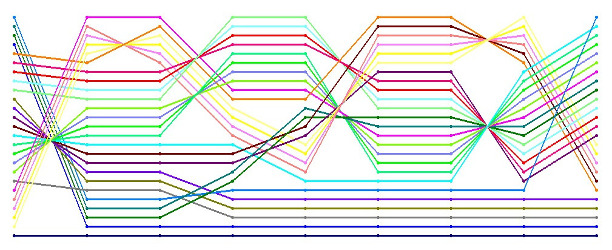
\includegraphics[width=0.6\textwidth]{images/sandyna}
\caption{Výstup z programu Michaely Sandalovej, Zdroj: \cite{biowiki}}\label{obr:sandyna}
\end{figure}
Naša práca čerpá inšpiráciu z programu Michaely Sandalovej, ktorý zobrazoval preusporiadania postupnosti génov - obrázok \ref{obr:sandyna}.